\Chapter{Több étterem, több futár, több kiszállítás esete}

\Section{A probléma megfoglmazása}

Ez az eset tisztán leírja a több lerakatos több ügynökös utazó problémát. Jelen esetben tisztázni kell, hogy a futárok különböző éttermekből indulnak ki. Próbálnak keresni egy olyan utat, aminek költésége viszonylag kicsi, tehát a közeli helyekhez tartozó csomagot veszik csak fel és szállítják ki. Ezt követően a legközelebbi kiszállítási helyet vizsgálják. Figyelembe veszik a szükségesen meglátogatni kívánt étterem körüli kiszállítási helyket és ez alapján választják meg az útjukat. Amennyiben ez az út túl költésges lenne, akkor próbál keresni egy másikat célt, aminél kevesebb út befektetésével több címet tud meglátogatni. Mindezek mellett, hogy a folyamatban ne legyen többszöri meglátogatás, a futároknak tudniuk kell, hogy ki hol járt már, hol történt meg a kiszállítás sikeresen.

\begin{figure}[h!]
\centering
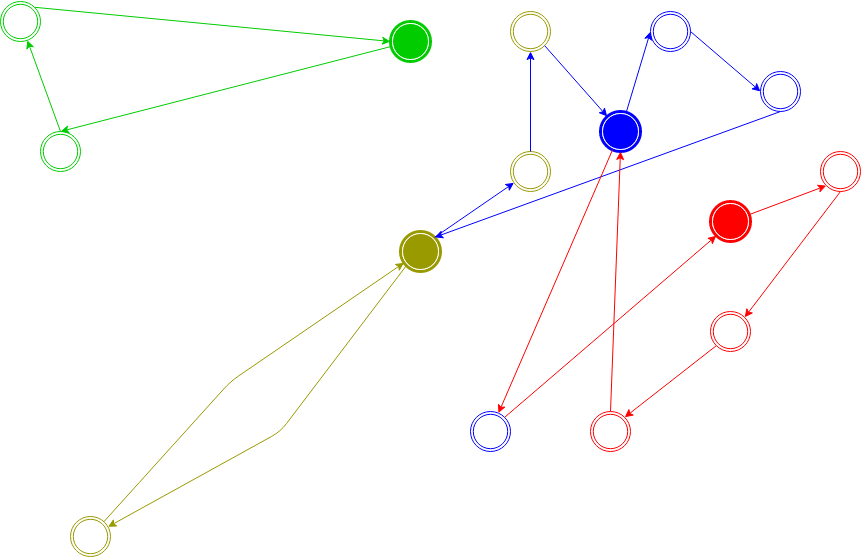
\includegraphics[scale=0.45]{images/model5.png}
\caption{Több étterem, több futár, több kiszállítás modellje}
\label{fig:model5}
\end{figure}


\Section{A probléma megoldása}

Első lépésként random pontokat kell generálnunk. Ezek jelképezik majd a kiszállítási helyeket. Ezt követően meg kell határoznunk az éttermek számát, majd legenerálni őket véletlenszerű helyekre. Később meg kell határoznunk egy átlag távolságot, ami a különböző kiszállítási pontok közötti távolságok átlagának felel meg. Nyílván kell tartanunk, hogy ki melyik étteremből rendelt, hogy ezáltal mindenképp az éttermet kelljen előbb meglátogatni, ha a csomag még egyik futárnál sincs. Tekintettel kell lenni a futárok aktuális helyezetére, hiszen ha elfogyott a csomagja keresni fogja a legközelebbi pontot ahova viheti majd a szállítmányt. Nélkülözhetetlen meghatározni a futárok útjait. Ehhez szükséges az előzőekben meghatározott átlag szakasz. A folymat felépítésére tekintettel szükséges egy fő ciklus mely a futárok számáig megy. Ezen belül megy egy másik ami a futár útjain megy végig. Ezen megoldás gyakorlati alkalmazása esetén lehetséges optimalizálni a kiszállításokat egy ilyen összetett modell esetén is.